\documentclass[letterpaper, 11pt]{article} 

\usepackage{graphics,graphicx}
\usepackage{multicol} 
\usepackage{parskip}
\usepackage{amsmath}
\usepackage{multirow}
\usepackage[utf8]{inputenc}
\usepackage{fancyhdr}
\usepackage[title]{appendix}
\usepackage{wasysym}
\usepackage{url}
\usepackage{subcaption}

\usepackage[font=footnotesize,labelfont=small]{caption}
\captionsetup{width=0.85\linewidth}

\RequirePackage{geometry}
\geometry{margin=2cm}

\setlength{\parskip}{0.2cm}
\setlength{\parindent}{0pt}


\title{Lab Report 6: Edge-Triggered Flip-Flop}
\author{
Tai Duc Nguyen \\
ECEC 471: Introduction to VLSI
}
\date{\today}

\begin{document}

\maketitle


%----------------------------------------------------------------------------------------
%	ABSTRACT
%----------------------------------------------------------------------------------------


\rule{\textwidth}{1pt}

\begin{abstract}
	A Flip-Flop is a circuit device that has two stable states, in which information can be stored. This circuit can be triggered to change its state by applying one or more control inputs. For this reason, the Flip-Flop is a basic storage element, used in many sequential circuits. In this laboratory report, the design, layout and simulation of an Edge-Triggered D-Flip-Flop is created in Cadence Virtuoso Layout and Cadence Virtuoso Schematic Editor.
\end{abstract}

\rule{\textwidth}{1pt}

\section{Initial Simulation and Results}
\label{sec:init_sim}

%\begin{multicols}{2}
The design for this experiment's Edge-Triggered D-Flip-Flop (DFF) is composed of standard gates: Inverter, 2-input NAND and 3-input NAND. Since the data can only be stored on a rising clock tick, the equation for the DFF is:

\begin{equation}
Q=\begin{cases}
1, & \text{Data if rising edge of Clock}.\\
0, & \text{else keep previous data}
\end{cases}
\end{equation}

From this equation, a well known schematic for the D-Flip-Flip is shown in Figure \ref{fig1}:

% Include Schematic Illustration of DFF
\begin{figure}[htb!]
	\centering
	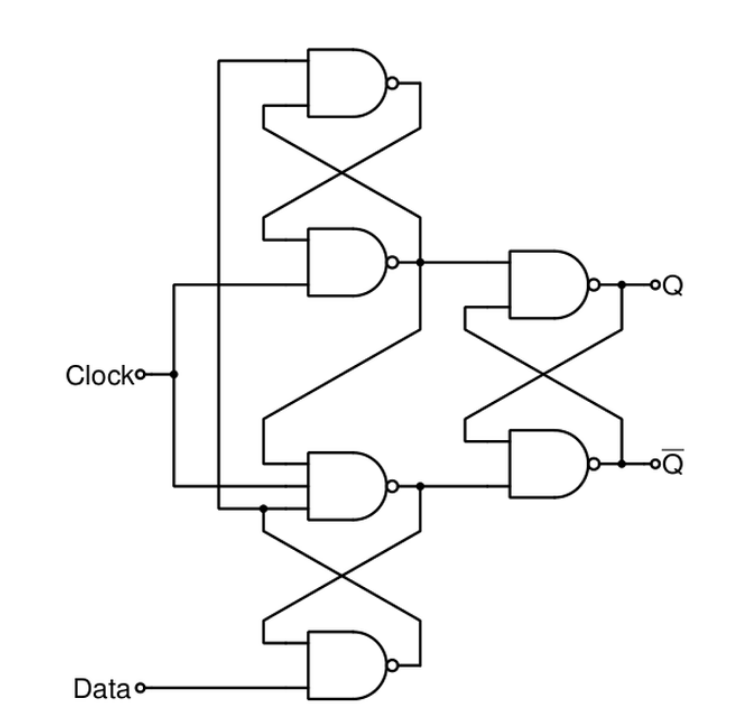
\includegraphics[width=0.3\linewidth]{dff_schematic_illustration.png}
	\caption{Schematic Illustration of the DFF}
	\label{fig1}
\end{figure}

This exact schematic is simulated on Cadence's Virtuoso Schematic Editor (in Figure \ref{fig2}):

% Include Schematic of DFF
\begin{figure}[htb!]
	\centering
	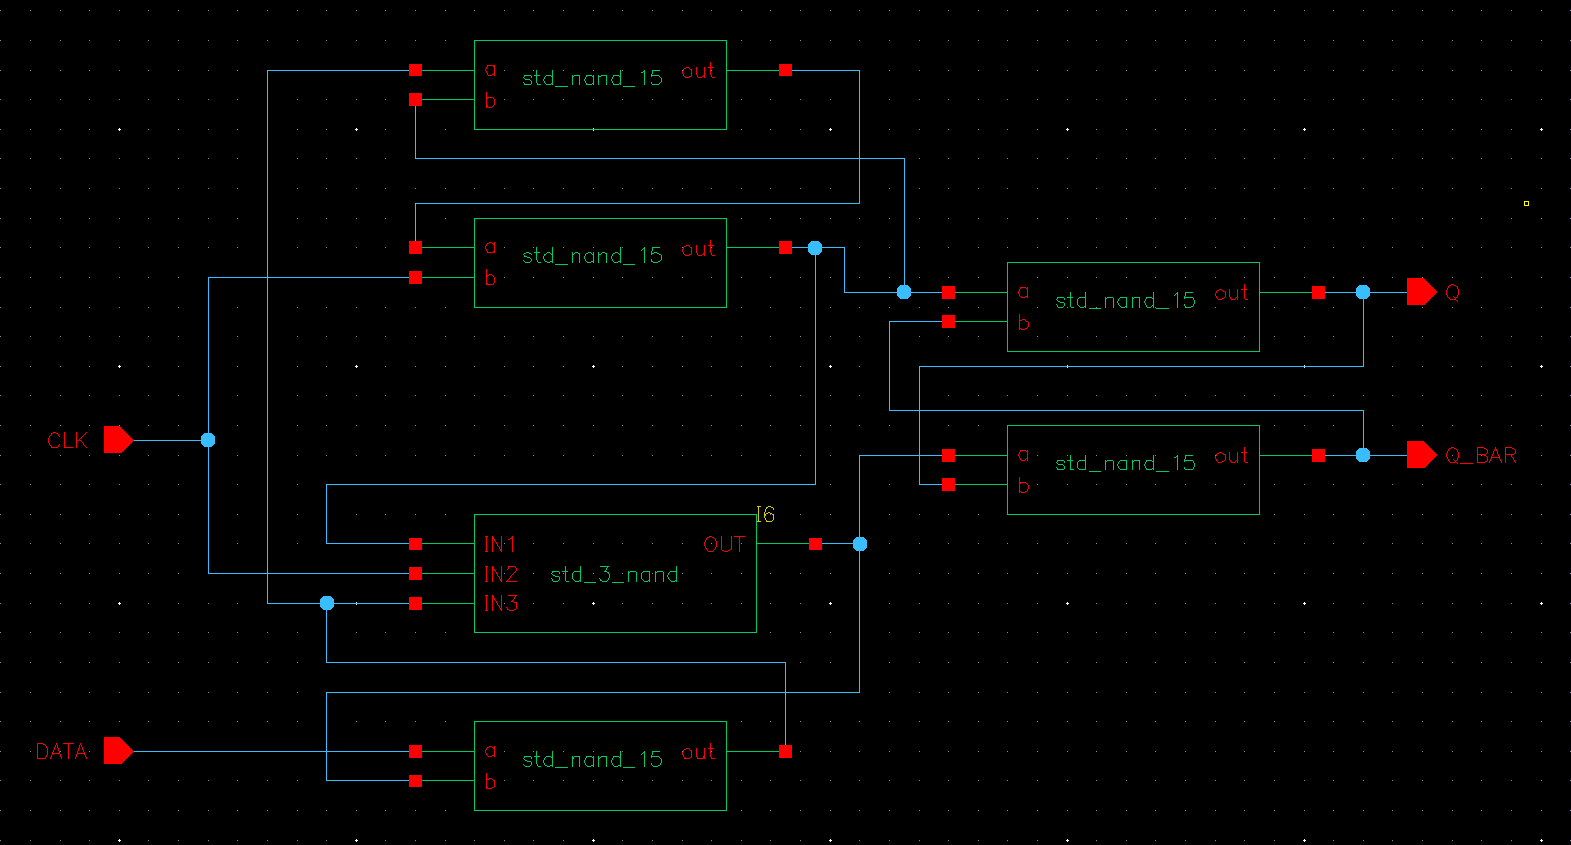
\includegraphics[width=1.0\linewidth]{dff_schematic.png}
	\caption{Schematic of the DFF in Cadence's Virtuoso Schematic Editor}
	\label{fig2}
\end{figure}

Since the DFF above contains inverters, 2-input NANDs and a 3-input NAND, 01 3-input NAND gate had to be created (in addition to the 2-input NAND gate and the inverters in previous experiments) and simulated with Cadence (shown in Figure \ref{fig3a} and \ref{fig3b}).

% Include Schematic and Layout of the 3-input NAND gate\\
\begin{figure}[ht!]
	\centering
	\begin{subfigure}[b]{.4\linewidth}
		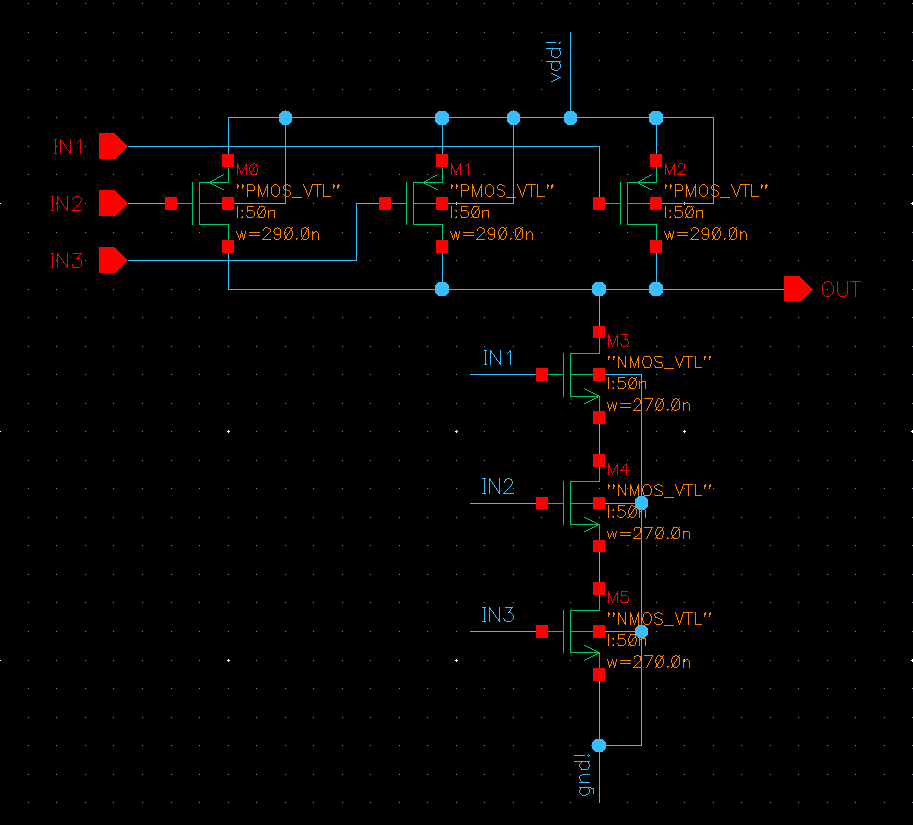
\includegraphics[width=\textwidth]{nand3_schematic.png}
		\caption{3-input NAND gate schematics}
		\label{fig3a}
	\end{subfigure}
%	\hskip2em
	\begin{subfigure}[b]{.3\linewidth}
		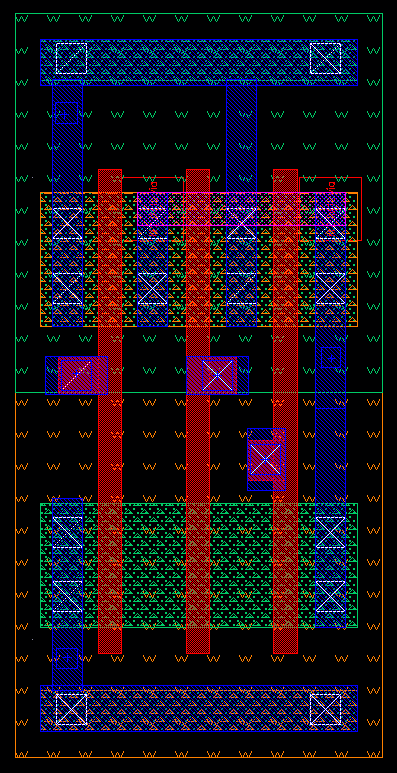
\includegraphics[width=\textwidth]{nand3_layout.png}
		\caption{3-input NAND gate layout}
		\label{fig3b}
	\end{subfigure}
	\caption{3-input NAND gate schematic and layout designs}
\end{figure}

The transient simulation results from the DFF above to verify the functionality of the D-flip-flop is shown below, in Figure \ref{fig4}

% Include initial transient of DFF
\begin{figure}[htb!]
	\centering
	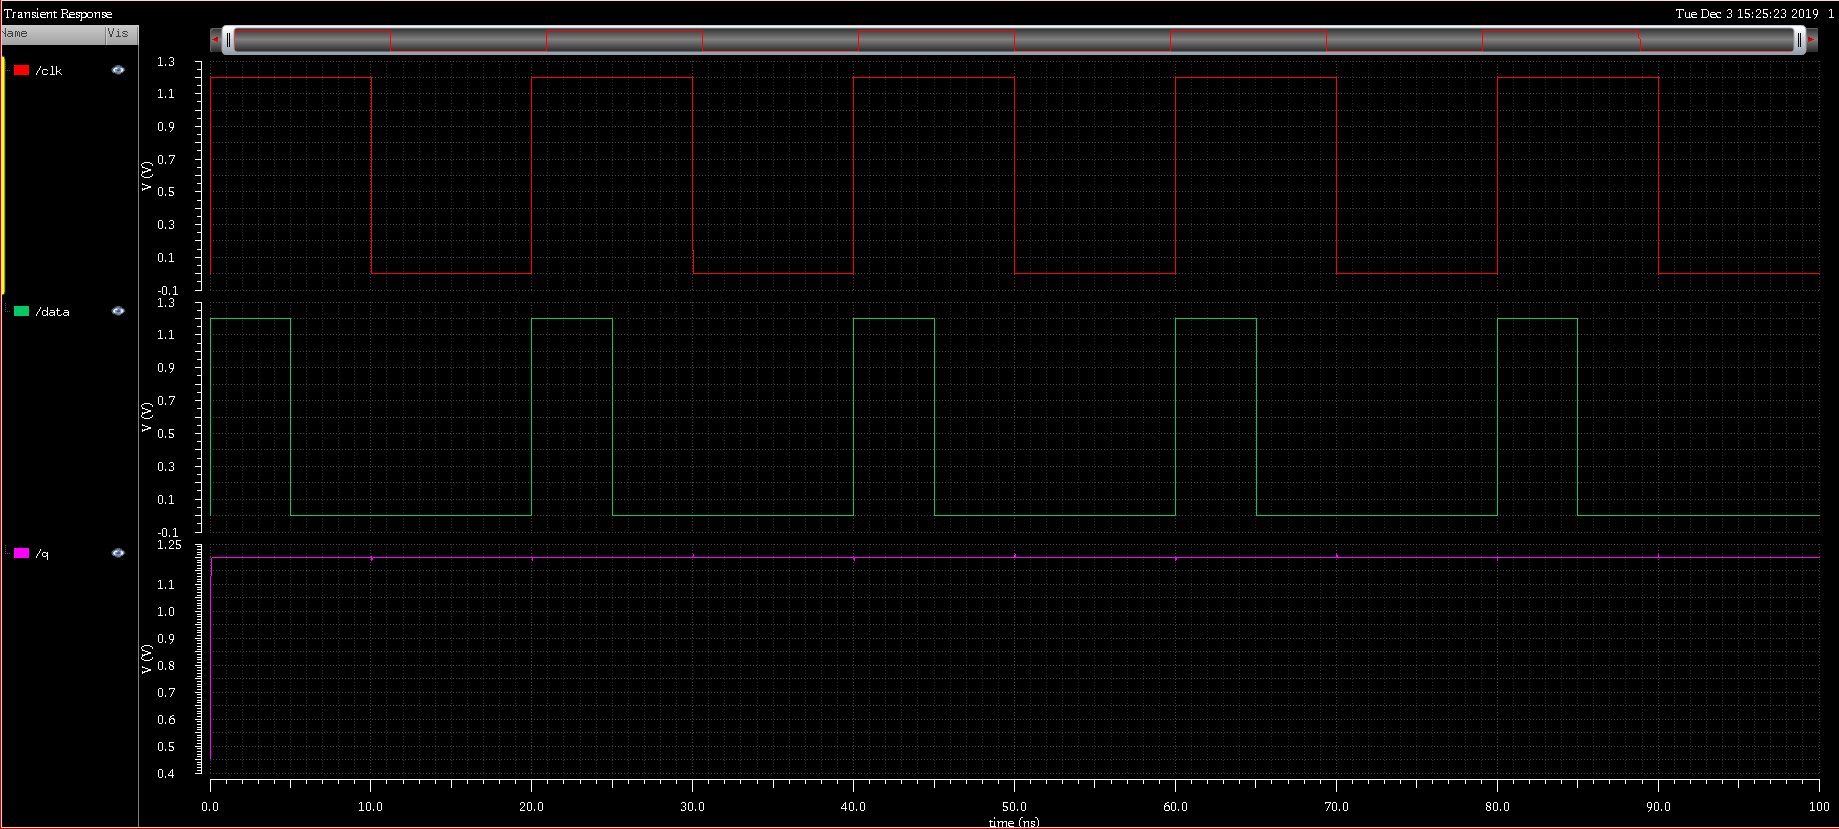
\includegraphics[width=1.0\linewidth]{dff_transient_init.png}
	\caption{Initial transient simulation result of the DFF}
	\label{fig4}
\end{figure}

\section{DFF's Device Characteristics}
\label{sec:device_char}
In order to take a closer look at the DFF created above, its setup time, hold time, rise/fall time and propagation delay is measured. Measuring the device's setup time requires Cadence's Parameter Analysis Tool, which does a parameter sweep over the delay of the DATA signal. As discovered, this DFF has a negative setup time due to its own wiring (the clock signal is processed earlier than the data signal). Hence, the DATA signal is shifted to the right until the output cannot register a 1 -- the shifted distance in time will be recorded as the setup time for this device (Figure \ref{fig5})

% Include setup time of DFF
\begin{figure}[htb!]
	\centering
	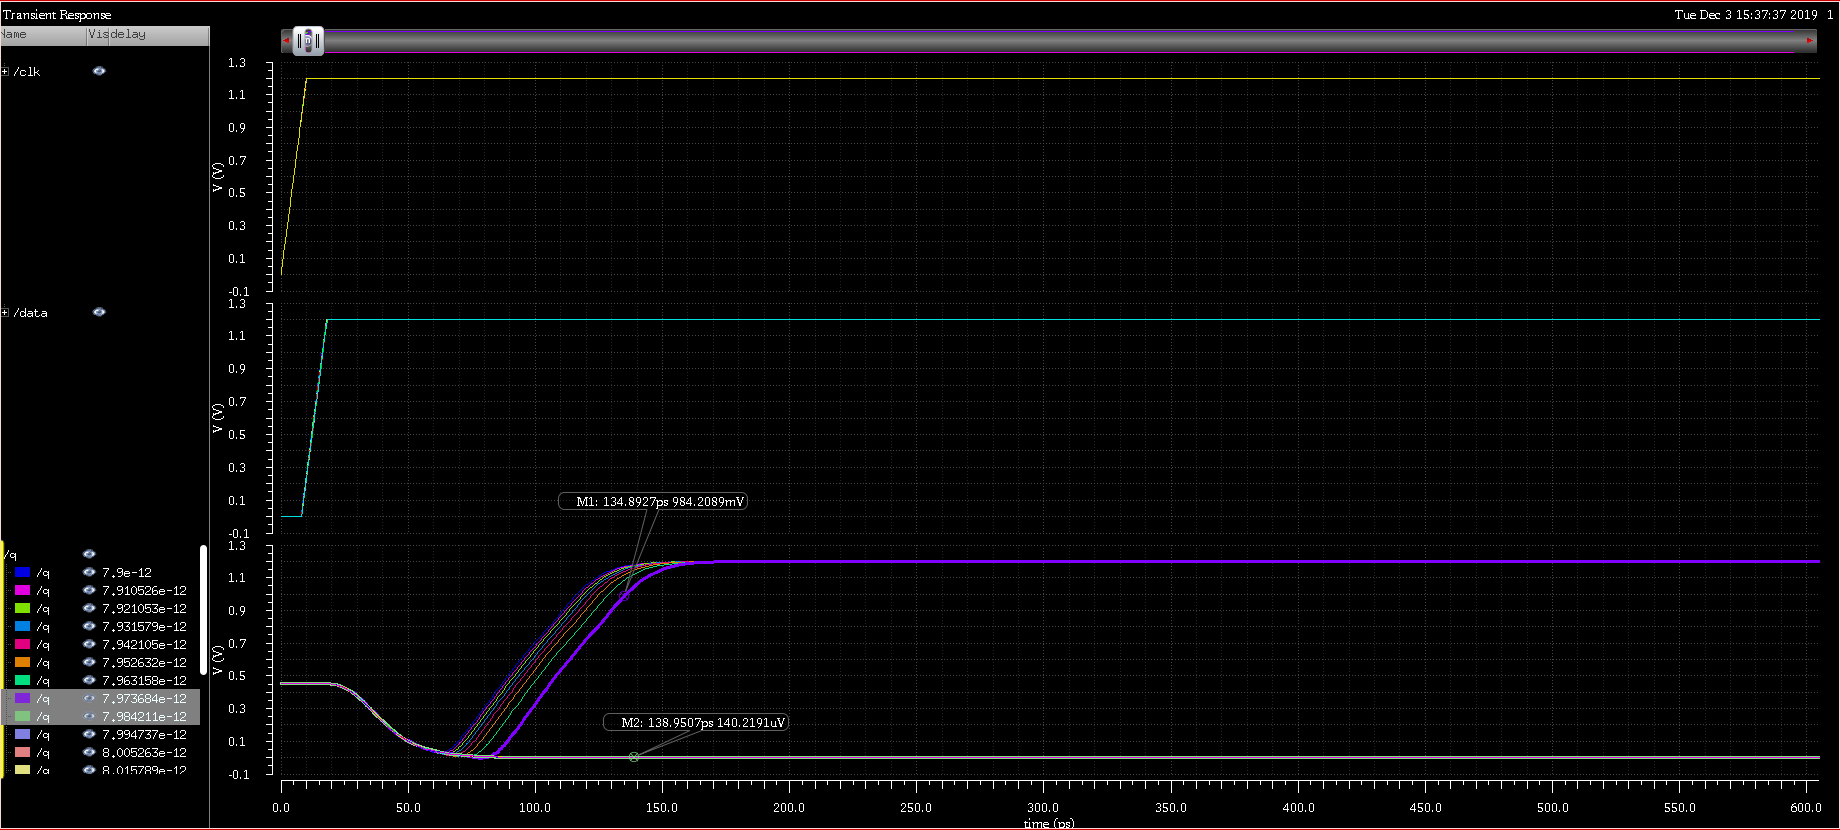
\includegraphics[width=0.95\linewidth]{dff_transient_sweep_setup_time.png}
	\caption{Parametric Sweep of the Delay to find DFF's Setup Time}
	\label{fig5}
\end{figure}

From the simulation above, the setup time for the DFF is:

% Calculate setup time
$t_{setup} = 7.973684e-12 = 7.97ps$

Similarly, the hold time of this DFF is obtained by making the pulse width of the DATA signal smaller and smaller until the output cannot register a 1 -- the smallest pulse width of the DATA signal is recorded as the hold time for this device (Figure \ref{fig6})

% Include hold time of DFF
\begin{figure}[htb!]
	\centering
	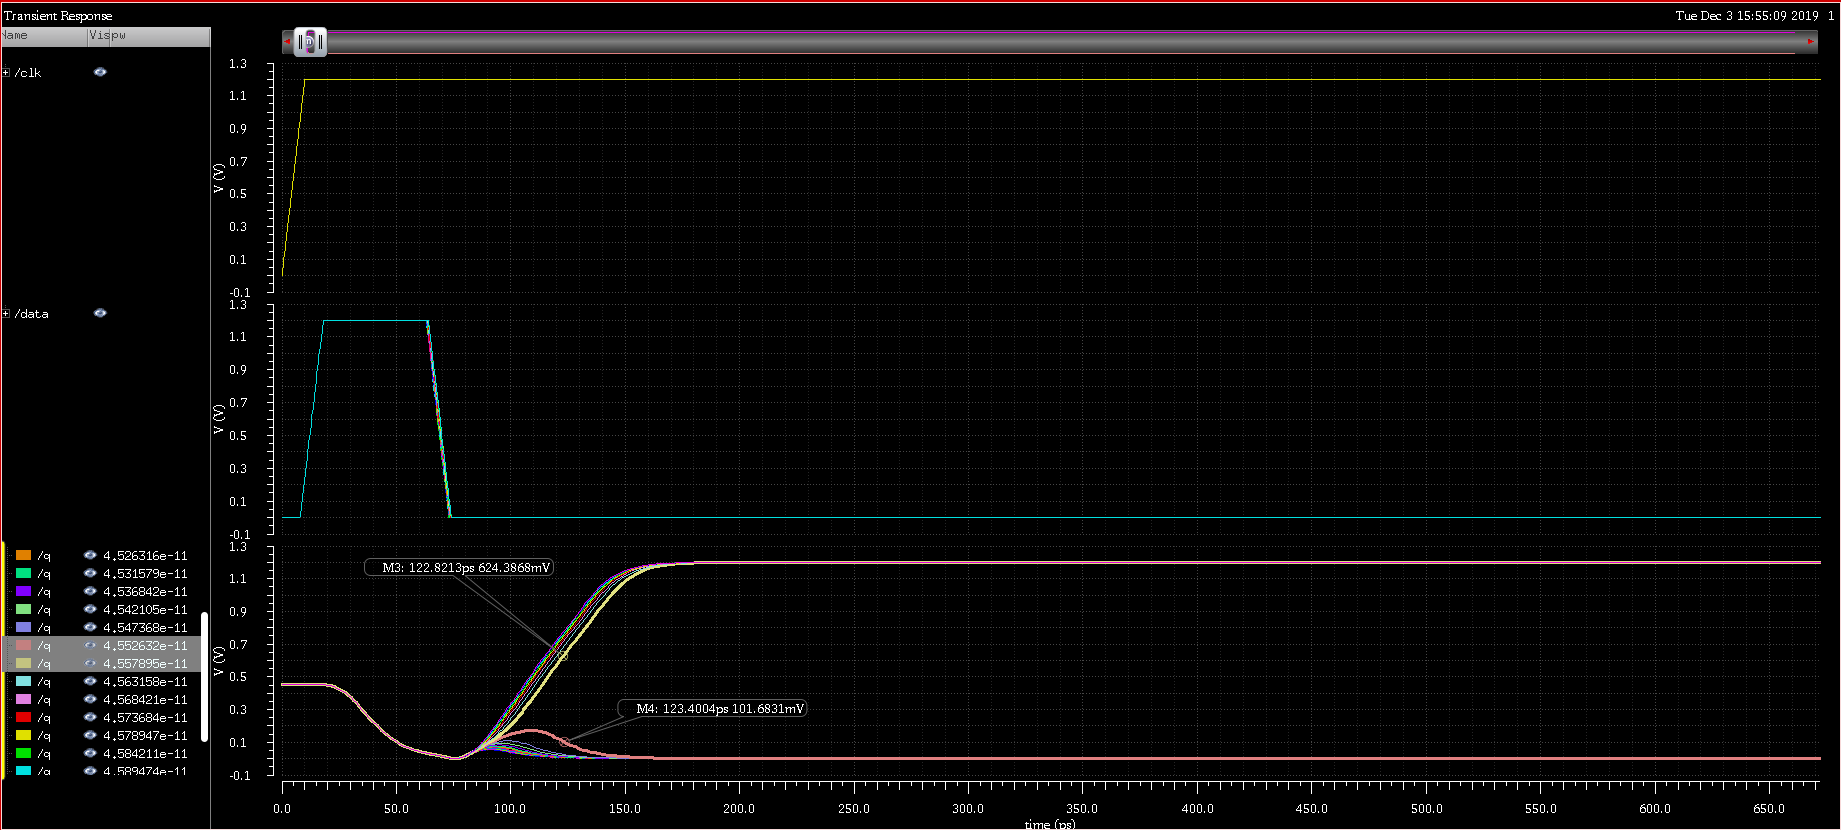
\includegraphics[width=0.95\linewidth]{dff_transient_sweep_hold_time.png}
	\caption{Parametric Sweep of the Delay to find DFF's Setup Time}
	\label{fig6}
\end{figure}

From the figure above, the hold time for the DFF is:

% Calculate hold time
$t_{hold} = 4.557895e-11 = 45.58ps$

In addition, The rise time, fall time and propagation delay of the DFF can be obtained and shown in Figure \ref{fig7a} and \ref{fig7b}.

% INclude rise fall prop delay of DFF
\begin{figure}[ht!]
	\centering
	\begin{subfigure}[b]{.95\linewidth}
		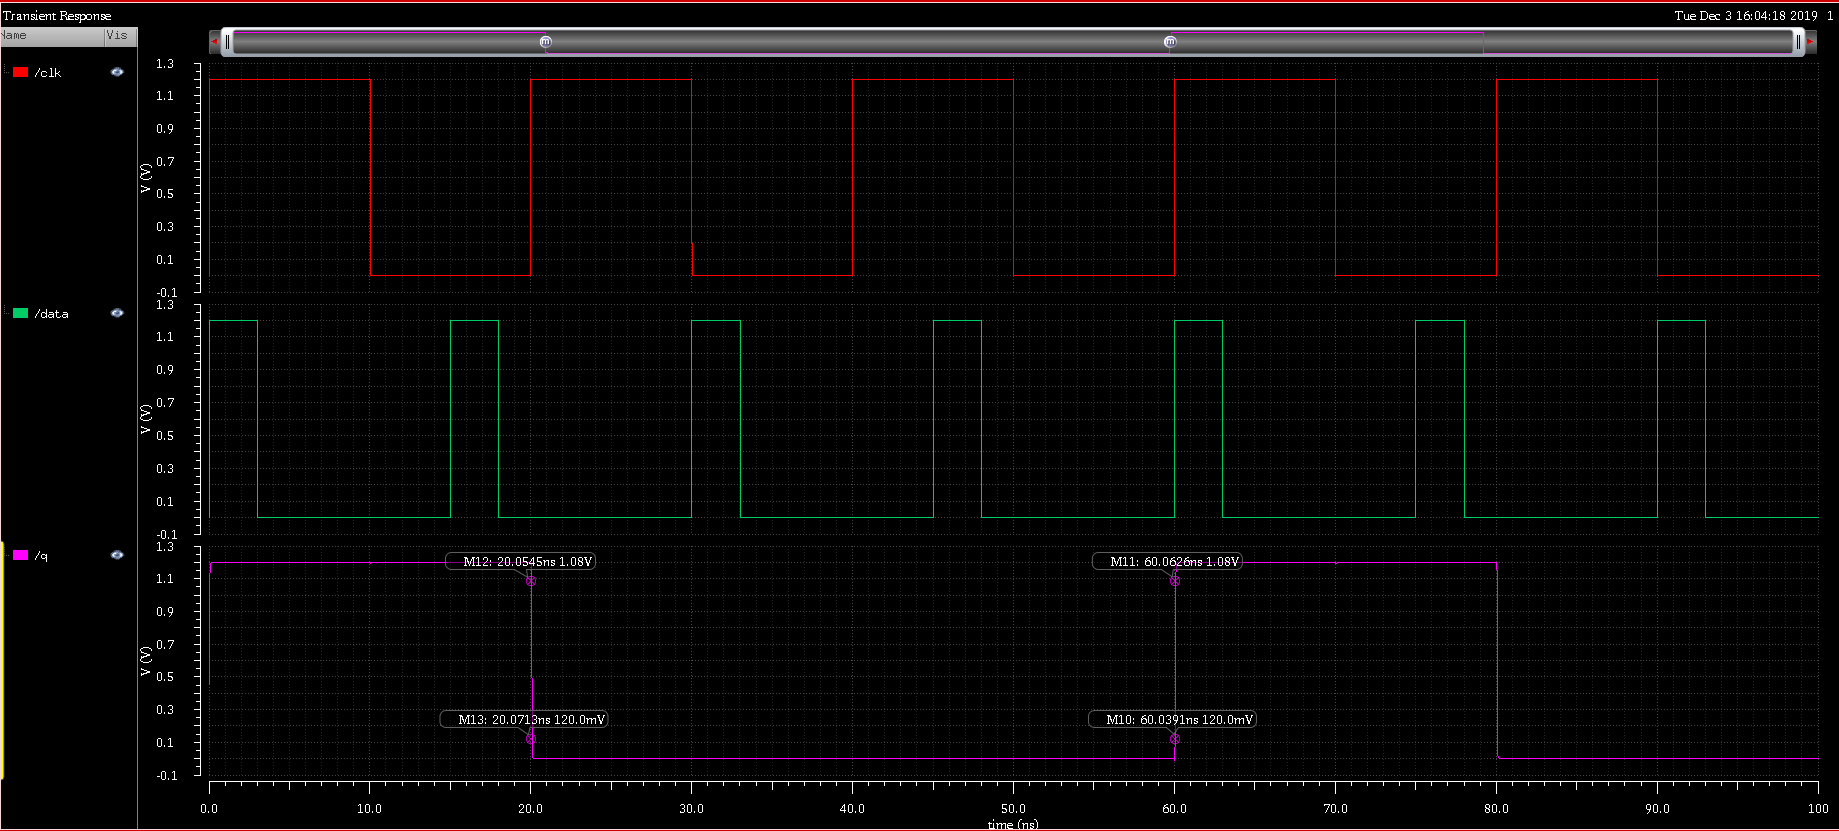
\includegraphics[width=\textwidth]{dff_rise_fall_time.png}
		\caption{DFF's rise and fall time}
		\label{fig7a}
	\end{subfigure}
	%	\hskip2em
	\begin{subfigure}[b]{.95\linewidth}
		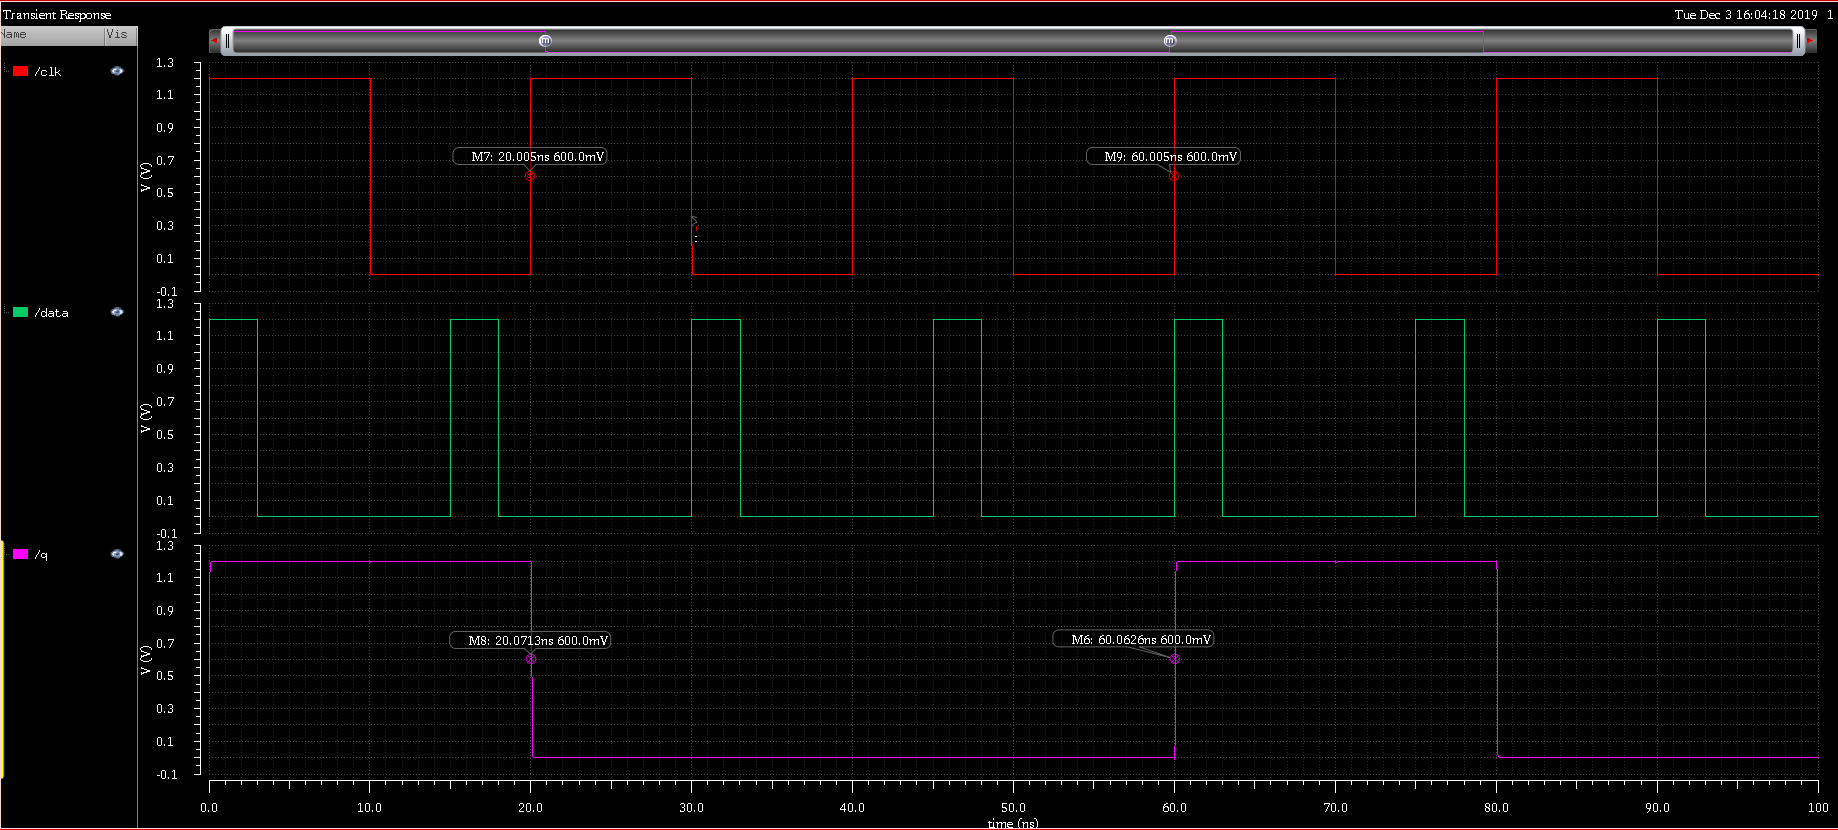
\includegraphics[width=\textwidth]{dff_prop_delay.png}
		\caption{DFF's propagation delay}
		\label{fig7b}
	\end{subfigure}
	\caption{Measurements of the DFF's rise/fall time and propagation delay}
\end{figure}

The rise time is:

$t_{rise} = 60.0626-60.0391 = 0.0235ns$

The fall time is: 

$t_{fall} = 20.0713-20.0545 = 0.0168ns$

The propagation delay is: 

$t_{pdr} = 60.0626-60.005 = 0.0576ns$

$t_{pdf} = 20.0713-20.005 = 0.0663ns$

$t_{pd} = (0.0576 + 0.0663)/2 = 0.06195ns$

\newpage
\section{Layout Design and Physical Verification}
\label{sec:layout_phys_verify}

The layout for the DFF is done with Cadence's Virtuoso Layout Suite and shown below in Figure \ref{fig8}:

\begin{figure}[htb!]
	\centering
	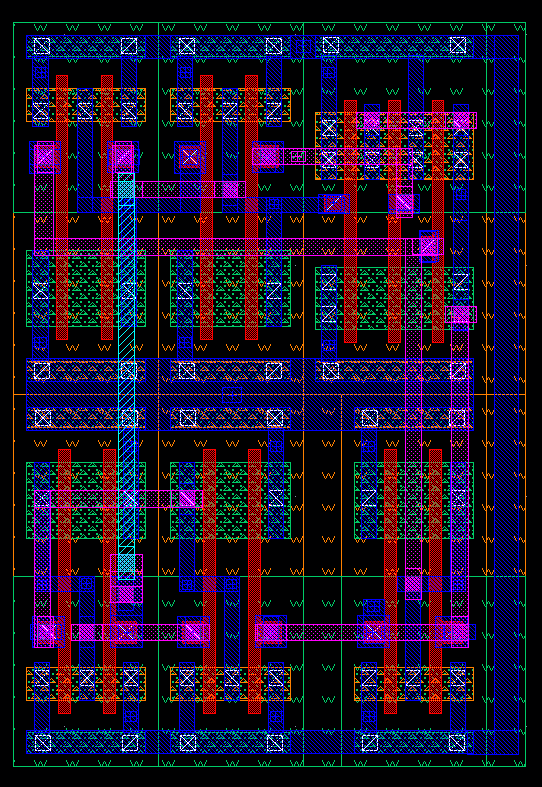
\includegraphics[width=0.6\linewidth]{dff_layout.png}
	\caption{DFF's Layout in Cadence's Virtuoso Layout Suite}
	\label{fig8}
\end{figure}

The DRC and LVS for this DFF is shown in Figure \ref{fig9a} and \ref{fig9b}:

\begin{figure}[ht!]
	\centering
	\begin{subfigure}[b]{.48\linewidth}
		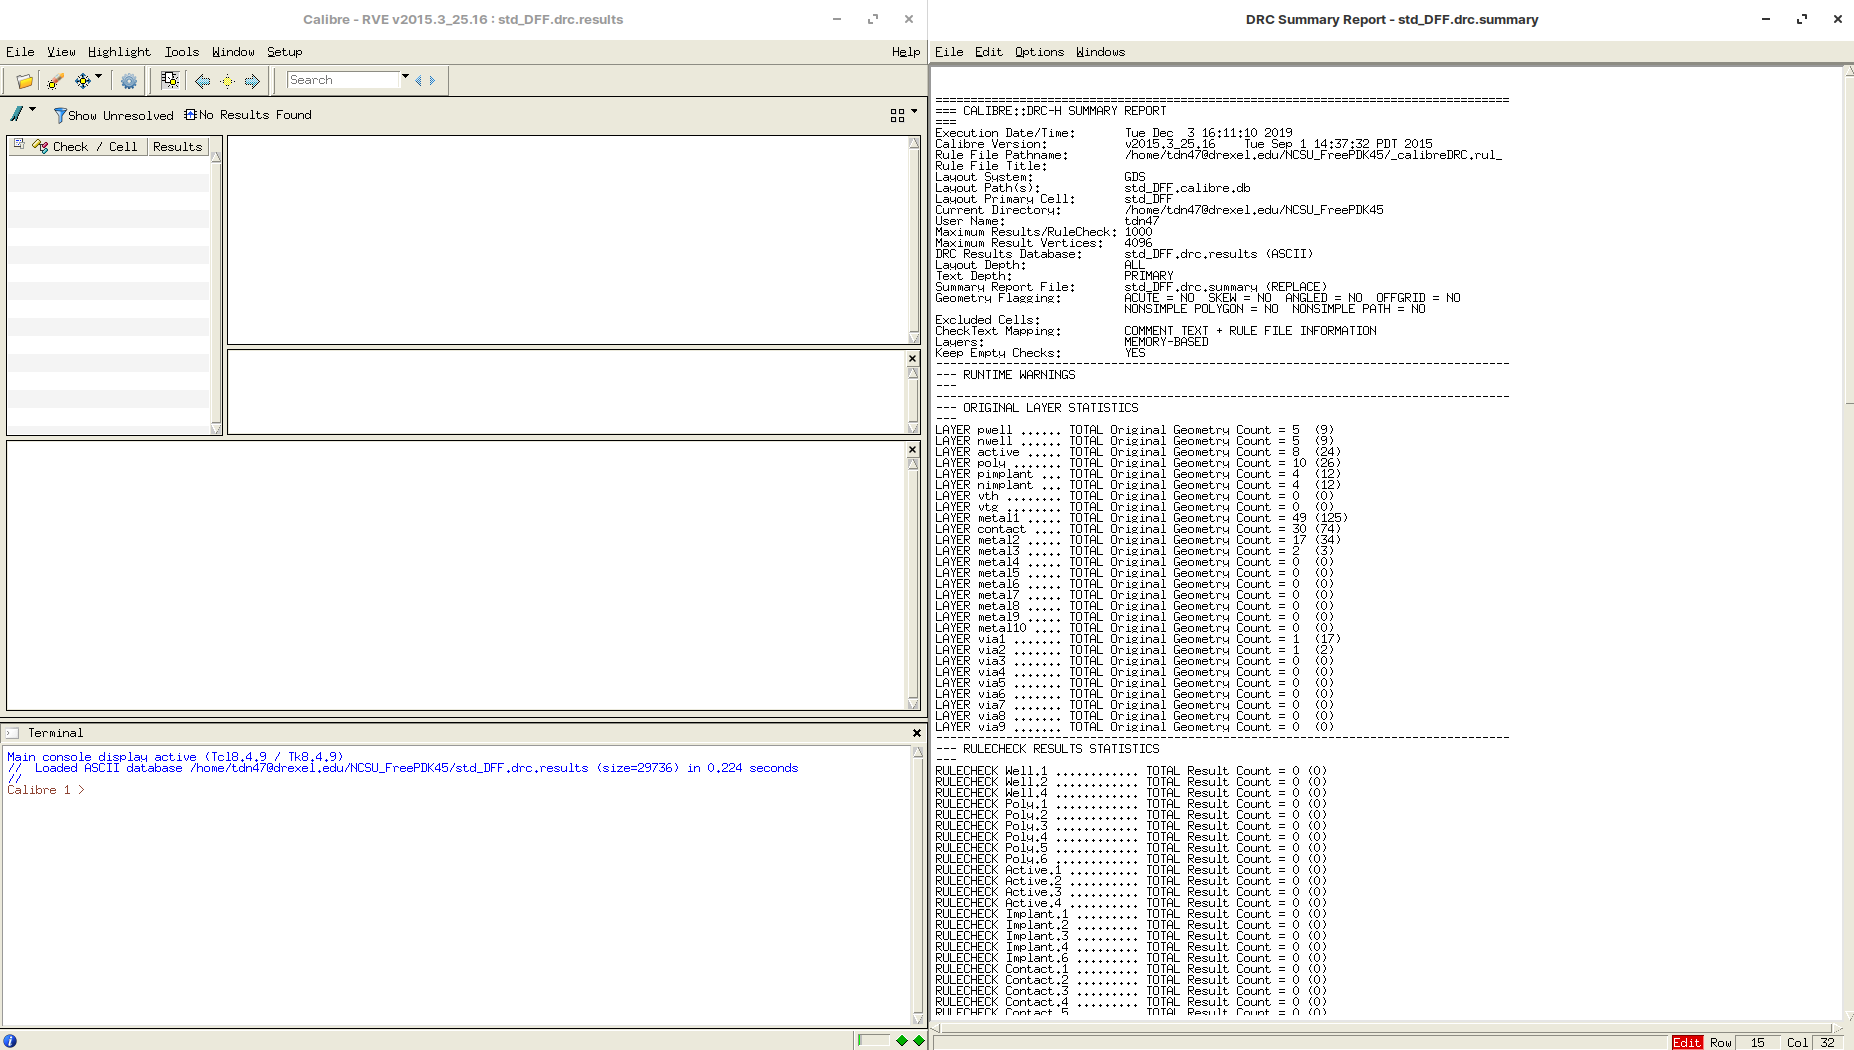
\includegraphics[width=\textwidth]{dff_drc.png}
		\caption{DFF's rise and fall time}
		\label{fig9a}
	\end{subfigure}
	%	\hskip2em
	\begin{subfigure}[b]{.48\linewidth}
		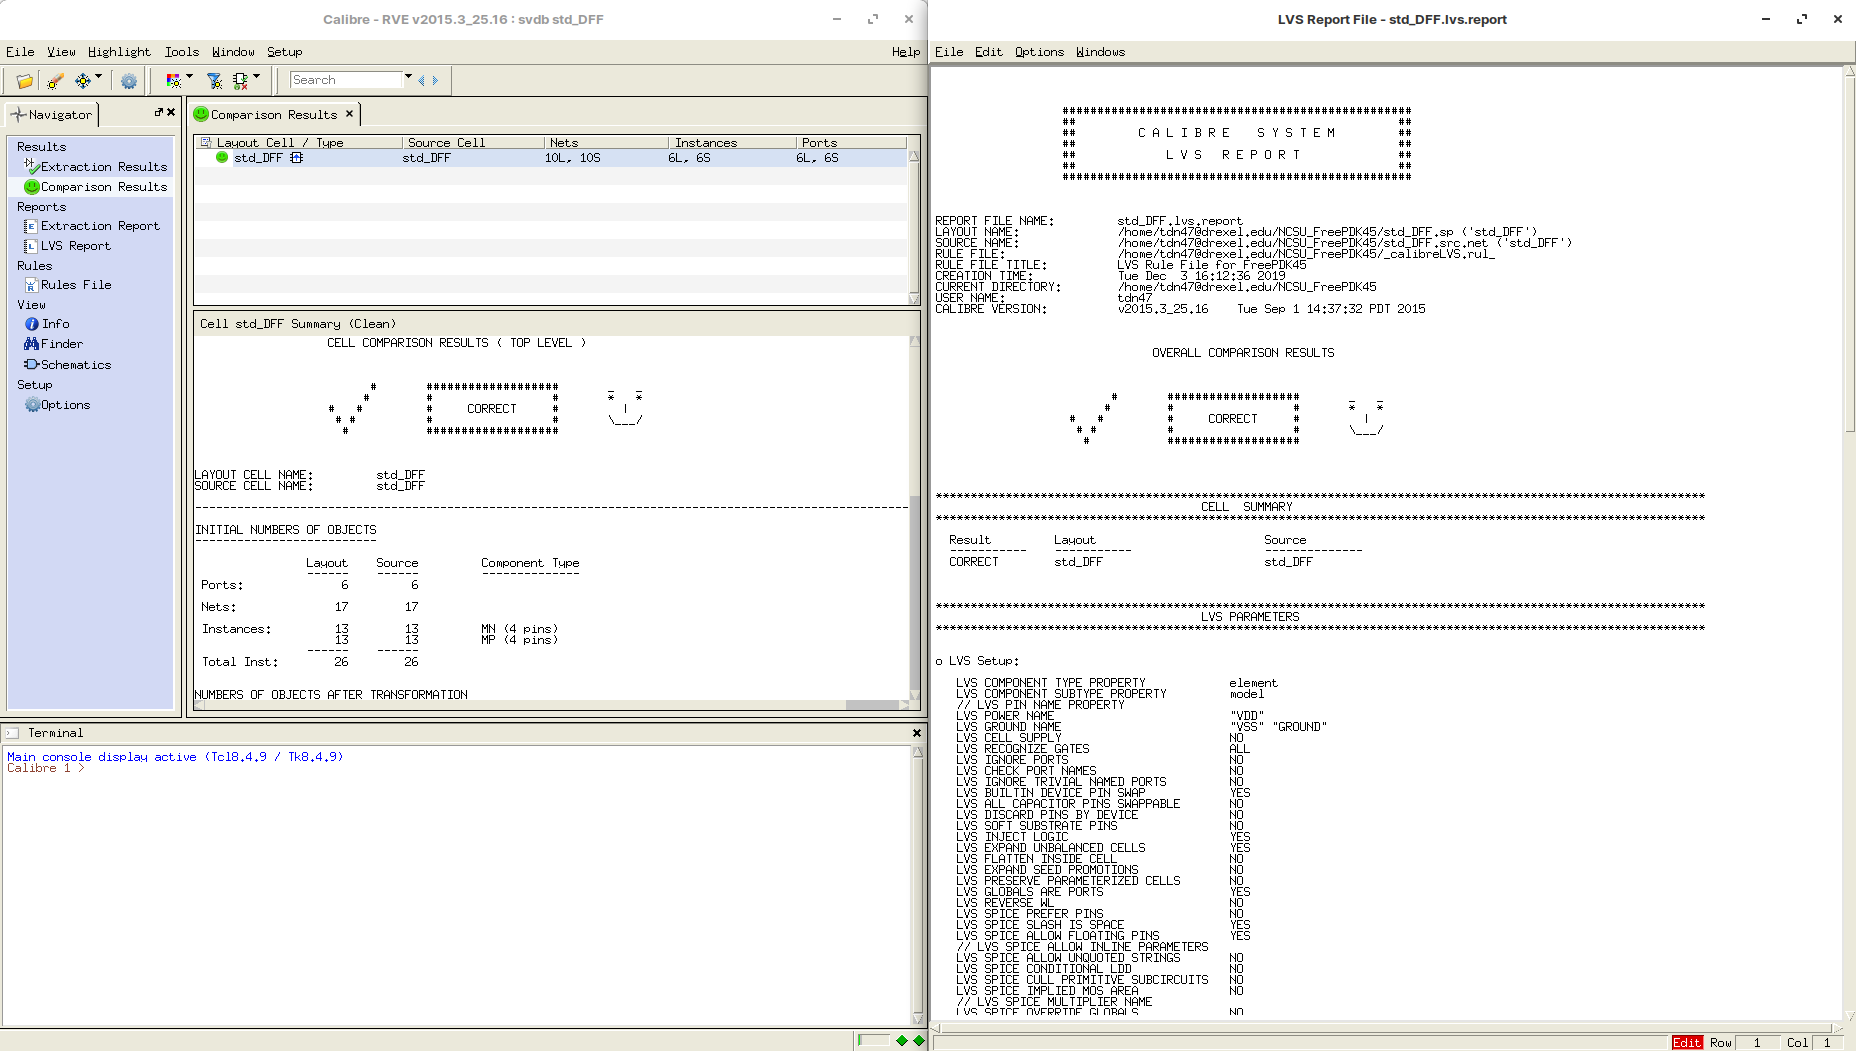
\includegraphics[width=\textwidth]{dff_lvs.png}
		\caption{DFF's propagation delay}
		\label{fig9b}
	\end{subfigure}
	\caption{Measurements of the DFF's rise/fall time and propagation delay}
\end{figure}

\newpage
\section{Discussion and Conclusion}
\label{sec:disc_n_concl}

The characteristic of the DFF created and simulated in this experiment is:

$t_{hold} = 4.557895e-11 = 45.58ps$

$t_{setup} = 7.973684e-12 = 7.97ps$

$t_{rise} = 60.0626-60.0391 = 0.0235ns$

$t_{fall} = 20.0713-20.0545 = 0.0168ns$

$t_{pd} = (0.0576 + 0.0663)/2 = 0.06195ns$

It is concluded that the setup time for this device is much smaller than its hold time, which means that the device needs the input DATA signal to be stable for much longer than it needs to be ready. 
The rise/fall time is not as symmetrical as it could be. This is due to the fact that the 3-input NAND gate in this design is not symmetrical. The propagation delay of the DFF is comparable to the 2-to-1 MUX in a previous experiment (0.06195ns vs. 0.06057ns).

\end{document}